%
% Complete documentation on the extended LaTeX markup used for Insight
% documentation is available in ``Documenting Insight'', which is part
% of the standard documentation for Insight.  It may be found online
% at:
%
%     http://www.itk.org/

\documentclass{InsightArticle}

\usepackage[dvips]{graphicx}
\usepackage{float}
\usepackage{subfigure}
\usepackage{amsmath} % for cases{}
\usepackage{graphicx}

%%%%%%%%%%%%%%%%%%%%%%%%%%%%%%%%%%%%%%%%%%%%%%%%%%%%%%%%%%%%%%%%%%
%
%  hyperref should be the last package to be loaded.
%
%%%%%%%%%%%%%%%%%%%%%%%%%%%%%%%%%%%%%%%%%%%%%%%%%%%%%%%%%%%%%%%%%%
\usepackage[dvips,
bookmarks,
bookmarksopen,
backref,
colorlinks,linkcolor={blue},citecolor={blue},urlcolor={blue},
]{hyperref}


\title{Small Hole Filling in ITK}

% 
% NOTE: This is the last number of the "handle" URL that 
% The Insight Journal assigns to your paper as part of the
% submission process. Please replace the number "1338" with
% the actual handle number that you get assigned.
%
\newcommand{\IJhandlerIDnumber}{3257}

% Increment the release number whenever significant changes are made.
% The author and/or editor can define 'significant' however they like.
\release{0.00}

% At minimum, give your name and an email address.  You can include a
% snail-mail address if you like.

\author{David Doria}
\authoraddress{Rensselaer Polytechnic Institute, Troy NY}


\begin{document}

%
% Add hyperlink to the web location and license of the paper.
% The argument of this command is the handler identifier given
% by the Insight Journal to this paper.
% 
\IJhandlefooter{\IJhandlerIDnumber}


\ifpdf
\else
   %
   % Commands for including Graphics when using latex
   % 
   \DeclareGraphicsExtensions{.eps,.jpg,.gif,.tiff,.bmp,.png}
   \DeclareGraphicsRule{.jpg}{eps}{.jpg.bb}{`convert #1 eps:-}
   \DeclareGraphicsRule{.gif}{eps}{.gif.bb}{`convert #1 eps:-}
   \DeclareGraphicsRule{.tiff}{eps}{.tiff.bb}{`convert #1 eps:-}
   \DeclareGraphicsRule{.bmp}{eps}{.bmp.bb}{`convert #1 eps:-}
   \DeclareGraphicsRule{.png}{eps}{.png.bb}{`convert #1 eps:-}
\fi


\maketitle


\ifhtml
\chapter*{Front Matter\label{front}}
\fi


% The abstract should be a paragraph or two long, and describe the
% scope of the document.
\begin{abstract}
\noindent
This code provides an implementation of a simple technique to fill small holes in an image. We use a multi-pass method that fills pixels on the border of a hole with the average of its non-hole 8-connected neighbors. This process is repeated until all holes are filled.

The code is available here: https://github.com/daviddoria/SmallHoleFiller

\end{abstract}

\IJhandlenote{\IJhandlerIDnumber}

\tableofcontents

%%%%%%%%%%%%%%%%%
\section{Introduction}
This code provides an implementation of a simple technique to fill small holes in an image. We use a multi-pass method that fills pixels on the border of a hole with the average of its non-hole 8-connected neighbors. This process is repeated until all holes are filled.

The code is available here: https://github.com/daviddoria/PoissonEditing

\section{Algorithm}
The algorithm we use is as follows:
\begin{itemize}
 \item Perform a raster scan of the image, looking for a pixel that is a hole.
 \item If the pixel has at least 1 valid 8-connected neighbor, set its value to the average of its valid neighbors.
 \item Do NOT mark this pixel as valid - it should not be considered ``known'' for the remainder of this pass through the image.
 \item Repeat this process (re-raster scan) until no more pixels are invalid.
\end{itemize}

It is important that we do not mark pixels as known for the current iteration. This would lead to a bias towards the colors of known pixels that occur earlier in the raster scan order. Using our method, larger holes are filled from all sides simultaneously. If we had marked new pixels as known during each pass, holes would be filled in a ``left to right, top to bottom'' fashion.

%%%%%%%%%%%%%%%%%
\section{Demonstration}
Figure \ref{fig:HoleFilling} shows an image with bright green pixels indicating invalid regions.

\begin{figure}[H]
\centering
\subfigure[Original image]{
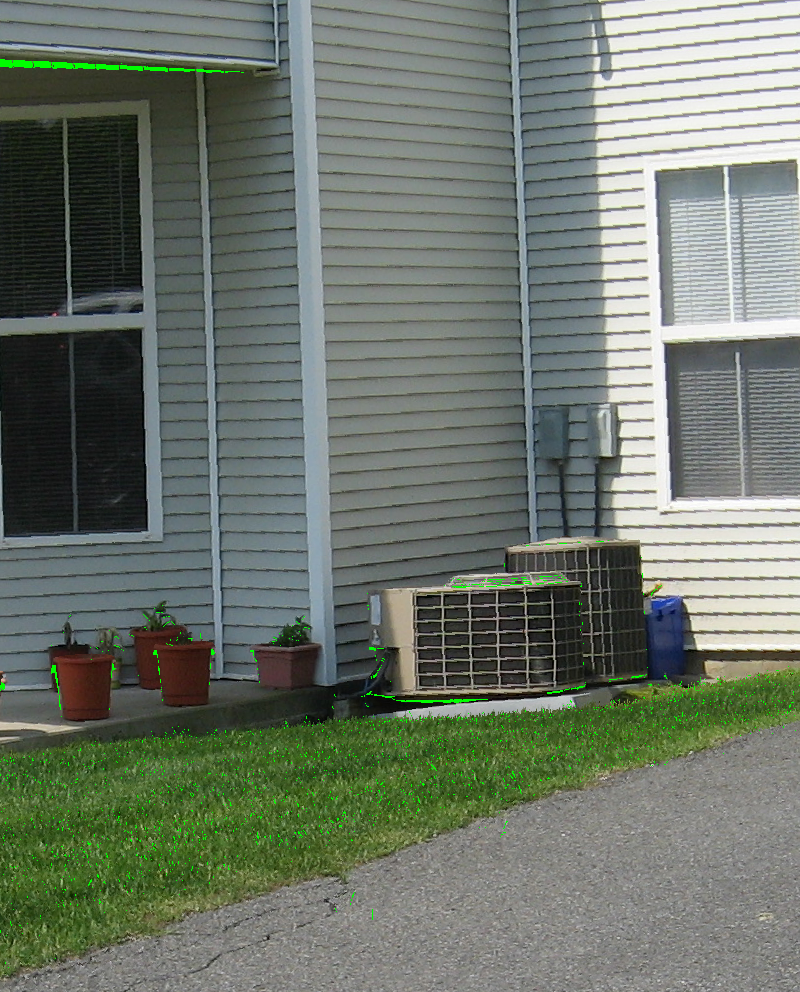
\includegraphics[width=0.3\linewidth]{images/input}
\label{fig:HoleFilling:original}
}
\subfigure[Filled image]{
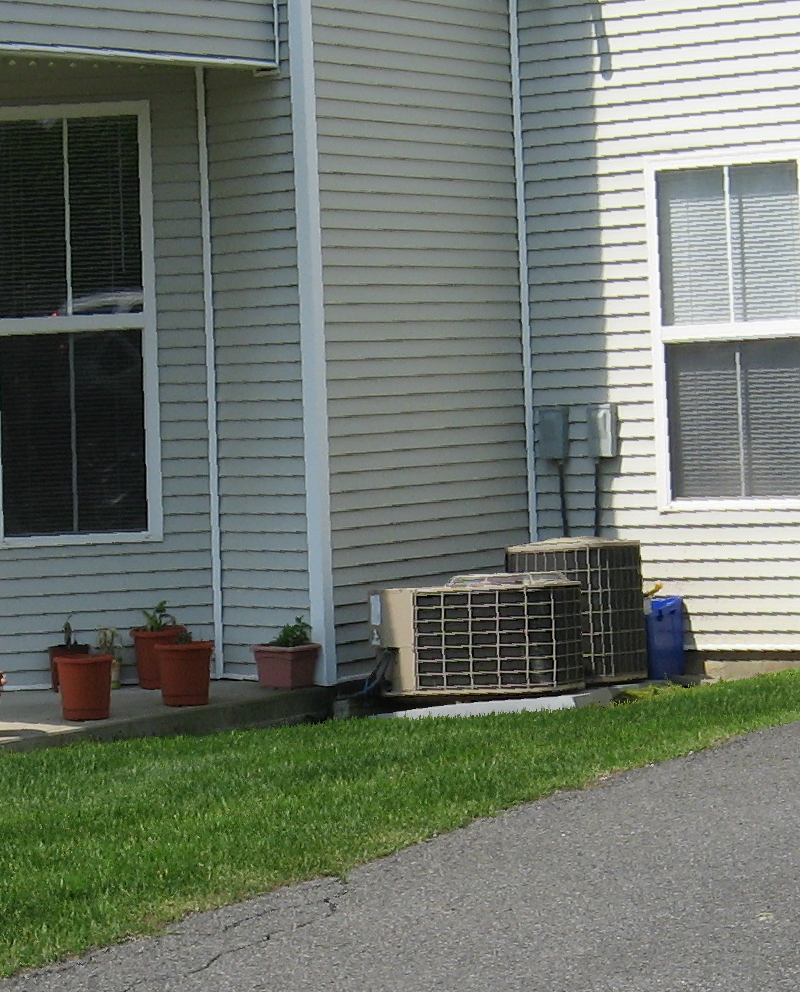
\includegraphics[width=0.3\linewidth]{images/output}
\label{fig:HoleFilling:output}
}
\caption{A demonstration of hole filling}
\label{fig:HoleFilling}
\end{figure}

%%%%%%%%%%%%
\section{Code Snippet}
The interface to the code is very straight forward.

\begin{verbatim}
  
  // Instantiate the hole filler class 
  SmallHoleFiller<ImageType> smallHoleFiller;

  ... read an image and pass it to the hole filler...
  smallHoleFiller.SetImage(reader->GetOutput());
  
  // Indiate which values in the image should be treated like holes
  smallHoleFiller.SetHolePixel(holePixelValue);
  
  // Perform the filling
  smallHoleFiller.Fill();
  
  // Write output
  ... setup a writer and pass it the output of the hole filler ...
  writer->SetInput(smallHoleFiller.GetOutput());
  
\end{verbatim}

%\bibliography{InsightJournal}
%\bibliographystyle{plain} % MUST include this line or will get ``undefined reference'' errors

\end{document}

